\documentclass[a4paper]{report}

\usepackage{graphicx}
\usepackage[english]{babel}
\usepackage[utf8]{inputenc}
\usepackage[T1]{fontenc}
\usepackage{ragged2e}
\usepackage{hyphenat}
\usepackage{lmodern}
\usepackage{fancyhdr}
\usepackage[toc,page]{appendix}
\usepackage{tabularx}
\usepackage{float}
\usepackage{gensymb}
\usepackage{amsmath}
\usepackage{pdfpages}

\begin{document}
    \centering
    \LARGE{\textsc{VIETNAM AVIATION ACADEMY}} \\
    \vspace{3mm}
    \normalsize{Department of Telecomunication - Electronics Engineering Technology} \\
    \vspace{3mm}
    \large{LOCATION IN HO CHI MINH CITY} \\
    \vspace{3mm}
    
\includegraphics[scale=0.3]{logo.jpg} \\
    \vspace{3mm}
    \normalsize{PROJECT REPORT:} \\
    \vspace{15mm}
    \huge{\textbf{"Circuit Remote Controlled Using Infrared Light"}} \\
    \vspace{20mm}
    \normalsize{Written by} \\
    \vspace{3mm}
    \large{\textit{Nguyen Van Anh Tuan}} \\ 
    \vspace{3mm}
    \textit{\large{Roll.No.1753020018}} \\
    \vspace{15mm}
    \textbf{\large{Under the guidance of}} \\
    \vspace{10mm}
    \centerline{\textbf{\large{Master Cao Xuan Kim Anh}}}

    % Lines down here to set footer and header. 
    \pagestyle{fancy}
    \fancyhf{}
    \rhead{Report Project 1}
    \lhead{CaptainJAV}
    \cfoot{\today}
    \renewcommand{\headrulewidth}{2pt}
    \renewcommand{\footrulewidth}{1pt}

    \newpage
    \centerline{\textbf{\huge{PREAMBLE}}} 
    \vspace{10mm}
    \begin{flushleft}
        In this day of advancement, we are indispensable remote control to control
        the devices we use every day as televisions, machines air conditioners, fan, etc.
        So how do remote controls work? Can control other objects in the distance? 
        Few know that the first remote control available during World War II. 
        Initially, people use RF technology (Radio Frequency) and then catch to start applying 
        IR (Infarred Remote) technology to the remote control. In today's life, we use 
        both types, however control remote use infarred in more often used. Let's see the principle operation 
        and construction of this remote control.
    \end{flushleft}
    \begin{flushright}
        \textbf{Auth. Nguyen Van Anh Tuan}
    \end{flushright}
    \thispagestyle{plain} % This command make this page have no header or footer.

    \newpage
    \tableofcontents

    \chapter{Introduction}
    \thispagestyle{fancy}
    \fancyhf{}
    \fancyhead[L]{CaptainJAV}
    \fancyhead[R]{Remote Controlled Using Infarred}
    \raggedright % Set all text to the left side.
    \rfoot{Page \thepage}
    \section{Preliminary introduce:} 
        With the current trend of modernization and industrialization, many modern technology 
        devices appear to help save time. We can mention as public technology of things 
        connected through the internet (Internet of Things) etc. But with expensive fees 
        are not suitable for the average consumer. From there, i founded simple solutions 
        with the same purpose and low cost.
        \linebreak
        \par In parallel, to supplement, to supplement the knowledge not studied 
        in school. From there, i selected "Remote Controlled Using Infarred" for the topic.
    \section{Objectives of the study:}
        To help reduce costs and supplement knowledge not researched at school.
    \section{Research Methods:}
        Find information on internet. \\
        Test on software. \\
        Construction circuit.


    \chapter{Find out theoretical related to the research}
    \thispagestyle{fancy}
    \fancyhf{}
    \fancyhead[L]{CaptainJAV}
    \fancyhead[R]{Remote Controlled Using Infarred}
    \rfoot{Page \thepage}
    \section{Application of remote controlled using infarred}
        Remote controlled now is using broadly, it use to controlled all wireless device. 
        Remotes and televisions are the best example for application of this recieve and transmitter 
        circuit. Or more application of this circuit. Beside that, we can see that remote controlled 
        can use with air conditioners, fans, or even use to turn on the lights in house...etc.
    \section{Define of Infarred (IR LED)}
        Infarred light (infarred ray) is the light we can't see it by our eyes, 
        they have wavelength from 700nm to 1mm. The infarred light have transmittion speed 
        is equal to lightspeed.
        \linebreak
        \par The infarred can transmit many signal channels. It is widely 
        applied in industry.
        \linebreak
        \par The amount of information that it can gain is 3 megabit/s. The 
        amount of information transmit with infarred light is many times larger 
        compared to the electromagnetic waves people still use.
        \linebreak
        \par Infarred rays are easily absorbed, poor penetration. In the word control 
        far by infarred, the beam emits a narrow, directed direction, so when recieve 
        must be in the right direction to use it.
        \linebreak
        \par Infarred wave have characteristics such as light (focusing through the lens, focal distance...). 
        Normal light and infarred light differ very clearly in light through the material.
        \linebreak
        \par Other than emitting invisible infarred light, IR Led look like a normal led and also
        works like a normal Led, it means it will consume 20mA and 3 Volts.
        \linebreak
        \par Besides that infarred is divided by wavelength into three main regions. However, follow the US classification is divided into 5 areas as follow: \\ 
        \vspace{3mm} 
        \begin{table}[ht]
            \centering
            \begin{tabular} { | p{1cm} | l | p{2cm} | p{2cm} | p{2cm} | p{3cm} | }
            \hline
            Name &Acronym &Wavelength &Frequency &Photon Energy &Featured \\ 
            \hline
            Near Infarred &NIR &750nm to 1.4$\mu$m &214-400THz &886-1653 meV &Determined by the absorption of water.Used in fiber optic telecomunications. \\ 
            \hline
            Short waves infarred &SWIR &1.4-3$\mu$m &100-214THz &413-886meV &Absorbed domestic increase significantly as of 1.45$\mu$m. Range 1.53-1.56$\mu$m is spectral region currently in use much in the far informed long road. \\ 
            \hline
            Medium waves infarred &MWIR &3-8$\mu$m &37-100THz &155-413meV &This band is called is thermal infarred, but it only detects slightly higher temperatures than body temperatures. \\ 
            \hline
            Long waves infarred &LWIR &8-15$\mu$m &20-37THz &83-155meV &This region is call "thermal infarred". \\ 
            \hline
            Far infarred &FIR &15-1000$\mu$m &0.3-20THz &1.2-83meV &See far infarred and far infarred laser. \\ 
            \hline
            \end{tabular}
            \caption{\label{tab:first}Classify Common of Infarred}
        \end{table}
    \section{Infarred receiver eye (TSOP-17xx)}
        It is an excellent line of infarred sensors for remote control applications. These infarred 
        sensors are designed to improve shielding electric interface. These devices are designed to 
        receive infarred rays from the infarred diode from a remote handset. 
        \linebreak
        \par TSOP 17xx is a part of the Photomodules family of infarred sensors modules miniature with PIN 
        photodiode and preamplification stage are placed in the shell epoxy. Its output is low and 
        gives +5V when off. Its output is demodulation to be able to decoded directly by the microprocessor. 
        Functions important modules include internal filter for PCM frequency capability. Compatible 
        with TTL and CMOS, low power consumption (5V and 5mA), immune to ambient light, anti-jamming, etc....
        \begin{table}[ht]
            \centering
            \begin{tabular} { | l | l | l | }
                \hline
                Number & Name & Description \\ \hline
                1 & Ground & Grounding \\ \hline
                2 & Vcc & Usually connect to +5V, maybe 6V \\ \hline
                3 & Signal & Output Signal \\
                \hline
            \end{tabular}
            \caption{\label{tab:second}Configuration of TSOP}
        \end{table}
        \par So, where do we use it?
        \linebreak
        \begin{itemize}
            \item The TSOP sensors is capable of reading the output signal from the remote control like 
            TV, home theater remotely etc... All the remote controls will work with a frequency of 38KHz and 
            this IC can pick up any processor IR signal handle them and provide output on PIN 3 (signal).
            \item Also, keep in mind that this TSOP-1738 series will only receive 38KHz infarred signals. 
            So almost all the remote control in our country will work in 38KHz.
        \end{itemize}
        \par Application of TSOP-1738:
        \linebreak
        \begin{itemize}
            \item Receiving infarred signal.
            \item Decode the remote signal.
            \item Analyze, reproduce or copy signals remotely.
            \item Receiver circuit for remote control.
            \item Remote control test circuit.
        \end{itemize}
    \section{IC 4017}
        Firstly, IC 4017 is the decimal counting IC, counting the clock. When we take IC clock count 
        pulse and output 10 corresponding to 1 pulse.
        \begin{figure}[ht]
            \centering
            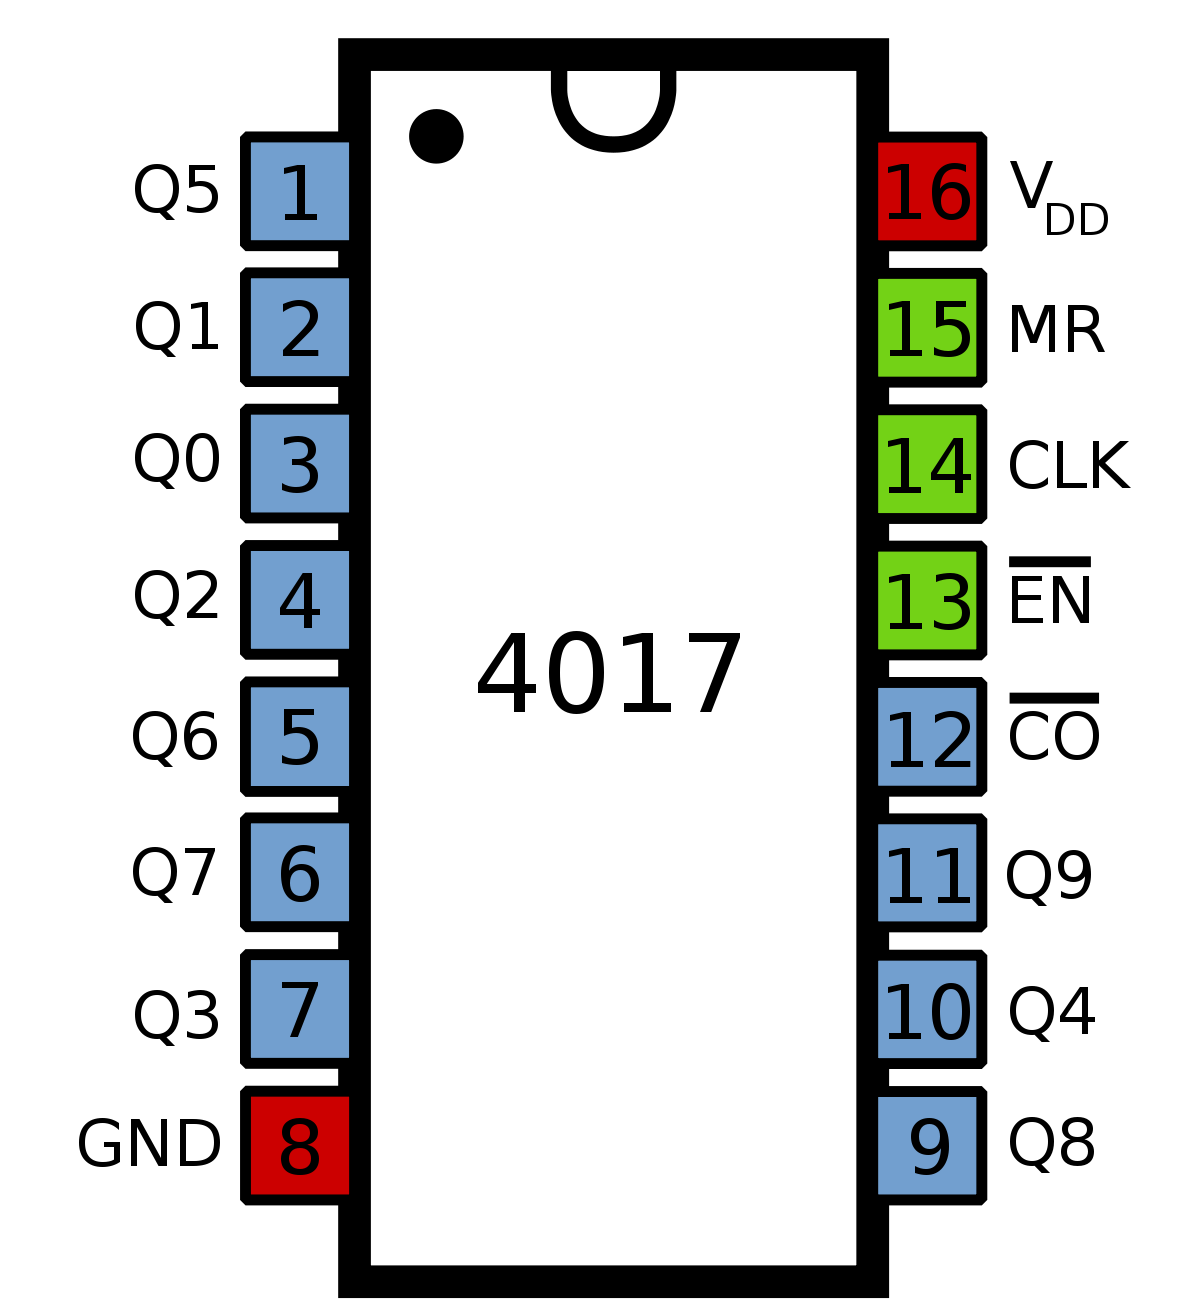
\includegraphics[width=0.5\linewidth]{4017.png}
            \caption{\label{fig:boat1}PIN chart of IC 4017}
        \end{figure}
        \begin{table}[ht]
            \centering
            \begin{tabular}{ | l | l | p{6cm} | }
                \hline
                Number & Name & Description \\ \hline
                1-7 and 9-11 & Output PINS Q0 to Q9 & 10 output, they are not in order, 
                so be careful when wiring \\ \hline
                8 & Vss or Ground & Grounding PIN \\ \hline
                12 & Carry out (CO) & The PIN to a high level after IC counting from 1-10. 
                Often used to trigger another count IC. \\ \hline
                13 & Clock Enable (EN) & PIN allowed. This positive PIN is low. When EN=0, 
                the circuit operates. \\ \hline
                14 & Clock & The counting circuit operates when there is a pulse from the 
                Clock PIN, which is positively edge-up, usually connected to another IC555 
                or quartz set to generate a pulse \\ \hline
                15 & Reset & Set output status to high \\ \hline
                16 & Vcc/Vdd & Connect to the source \\ 
                \hline 
            \end{tabular}
            \caption{\label{tab:third}Description of function of each IC 4017 PIN}
        \end{table}
        \newpage
        \par In summary we have the characteristics of the IC 4017 as follow:
        \linebreak
        \begin{itemize}
            \item 16-PIN CMOS decimal counter.
            \item Support 10 decoded outputs.
            \item Wide supply voltage range from 3V to 15V, usually +5V.
            \item Compatible with TTL (Transistor-transistor logic).
            \item Maximum frequency: 5,5MHz.
        \end{itemize}
        \par And what is application of IC 4017? That is:
        \linebreak
        \begin{itemize}
            \item This IC usually use in the counter circuit, timer circuit, LED matrix, LED chaser, 
            and almost the lost of other LED project.
            \item Use to make binary counter or binary decoder.
            \item Can be use to make splitters.
            \item Remote metering, cars, medical electronics.
        \end{itemize}
    \section{Quickview about clock pulse}
        In logic techniques, people use pulse signals (high and low) to operate. This signal is called a pulse. 
        \linebreak
        \par As you can see, the clock has an effect on the signal transmittion. Specifically, the higher 
        frequency of the clock, the faster amount of signal transmitted. 
        \linebreak
        \par For synchronous design systems, the clock is a global clock that allows all the components 
        on it to communicate and control with each other. 
        \linebreak
        \par As for the asynchronous setting system, the clock pulse is just a handshake pulse to 
        communicate between 2 components (local clock) with each other, absolutely no clock pulse for 
        the entire system. 
        \newpage
        \begin{figure}[ht]
            \centering
            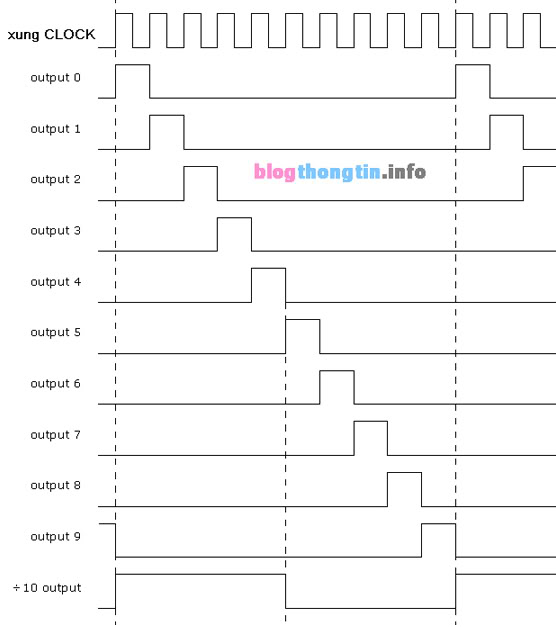
\includegraphics[width=0.5\linewidth]{n2.jpg}
            \caption{\label{fig:boat2}Output signal format according to pulse input signal of IC 4017}
        \end{figure}
        \par This is signal when IC is operated by an edge-up shock (the pulse from level 0 to level 1). 
        \linebreak
        \par PIN 13 (pin E) is the PIN that allow the IC to work, to activate this pin we have to connect 
        this pin to level 0 (also known as mass level).
        \linebreak
        \par MR pin or can be understood as Reset pin, when we give it a voltage of 1 (5V), the output Q 
        will be reset, the output Q0 is default at 1, the remaining outputs are at 0 if we do not need to use 
        the MR pin, we should connect this PIN to the mass. The diagram above we use MR pin to control 
        the 4th counting so we connect MR to Q4 pin.
        \linebreak
        \par CO pin used to connect with other IC 4017 depending on the design needs of each person, for 
        example when we need more counting of IC 4017 then we will use this pin (just connect the CO pin of this 4017 to the CLK pin of the next IC 4017).
        \linebreak
        \par As shown in the picture we see when the output pulse of the IC is simulated to a high level 
        (level 1) so continuously until the output of the IC and will return to the beginning and so on, 
        if it granted, it will be run continuously.
        \linebreak
    \section{IC NE555}
        \begin{figure}[ht]
            \centering
            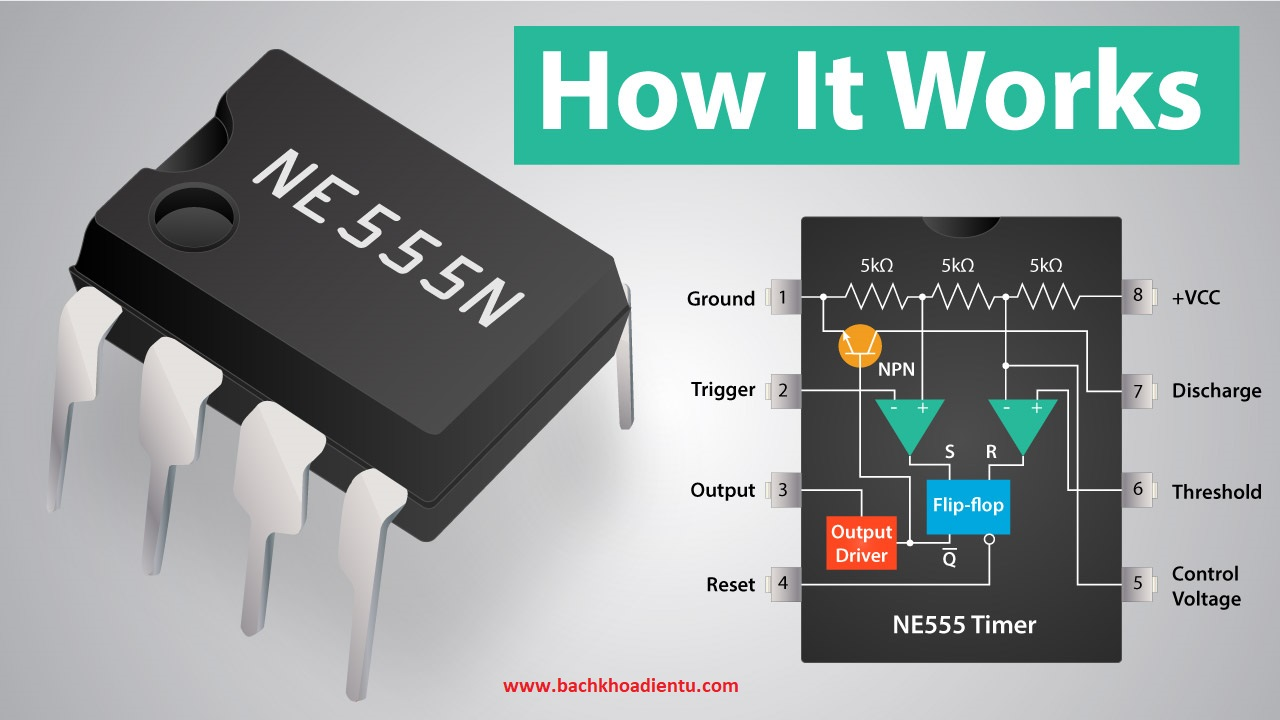
\includegraphics[width=0.5\linewidth]{555.jpg}
            \caption{\label{fig:boat3}Image and structure of IC NE555}
        \end{figure}
        \par NE555 Timer IC is an intergrated circuit (chip) used in a variety of timer, pulse generation, 
        and application oscillators. NE555 can be used to provide time lags, like an oscillators and as a 
        flip-flop element.
        \linebreak
        \par IC NE555 has been in 1972 by Signetics Corporation with 2 product lines SE555/NE555 and 
        is called time machine and is also the first available. It provides electronic circuit designers 
        with relatively cheap, stable cost.
        \linebreak
        \par Its structure is composed of OP-AMP comparing voltage, flip circuit and transistor for discharging 
        electricity like a image down here: 
        \begin{figure}[ht]
            \centering
            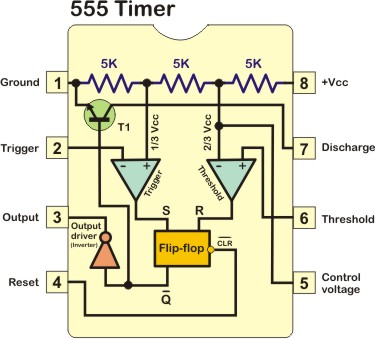
\includegraphics[width=0.6\linewidth]{inside_the_555_timer.jpg}
            \caption{\label{fig:boat4}Structure inside of NE555}
        \end{figure}
        \linebreak
        \par Depending on the manufacturer, NE555 has a different structure. Typically, the standard 
        NE555 include 25 transistors, 2 diodes, and 15 resistors on silicon processors installed in the 
        8-pin dual package (DIP-8). Variations include 556 (one DIP-14 combining tow complete 555s on one chip), 
        and 558/559 (both DIP-16 incorporating four reduced function timers on one chip).
        \linebreak 
        \par NE555 parts are temperature range from 0$^{\circ}$C to 70$^{\circ}$C and NE555 parts are 
        assigned the best temperature range from -55$^{\circ}$C to 125$^{\circ}$.
        \linebreak
        \par Low-power CMOS types of NE555 are also available, such as Intersil ICM7555 and Texas LM555, 
        TLC555, TLC551. The CMOS timer uses less power than the bipolar timer. The CMOS timer also causes 
        less noise than the dipole type when the output transitions.
        \begin{table}[ht] 
            \centering
            \begin{tabular}{ | l | l | l | p{7cm} | }
                \hline
                PIN & PIN Name & PIN direction & PIN purpose \\ \hline
                1 & GND & Ground & Supply voltage: 0V \\ \hline
                2 & TRIG & Input & Activate: when the voltage at this PIN decrease 1/2 of battery voltage CONT 
                (1/3 Vcc unless CONT have activate by outside signal). \\ \hline
                3 & OUT & Output & This is a push-pull output that is led to a low or high state (positive supply on the Vcc PIN minus about 1.7). \\ \hline
                4 & Reset & Reset & The time interval can be reset by bringing this PIN to GND, but the time does not 
                start again until this PIN rises to about 0.7V. This PIN overrides TRIG and Threshold. This PIN 
                is not used much, so it is often connected to Vcc to prevent electrical noise from causing repetition. \\ \hline
                5 & CTRL & Input & This PIN provides access to internal voltage (2/3 Vcc by default). Apply this 
                voltage to CONT, we can change the time characteristics of the device. \\ \hline
                6 & THRES & Input & Threshold: when this voltage at PIN is greater than the voltage at the CONT 
                PIN (2/3 Vcc), then the interval time ends. \\ \hline
                7 & DIS & Output & Discharge: this is the output of an open collector (OC), used to discharge 
                capacitors between intervals, in phase with the output. \\ \hline
                8 & Vcc & Source & The guaranteed voltage range of bipolar timers is usually 4.5-1.5V (some timers are specified for up to 16V or 18V), 
                although most will work as low as 3V. \\ 
                \hline
            \end{tabular}
            \caption{\label{tab:four}Describe the function of each IC NE555 pin}
        \end{table}
        \begin{table}[ht]
            \centering
            \begin{tabular}{ | l | l | }
                \hline
                Properties & Value \\ \hline
                Mounting type & Surface mount \\ \hline
                Timer type & Standard \\ \hline
                Package type & SOIC (Small Outline Intergrated Circuit) \\ \hline
                Number of timer & 1 \\ \hline
                Number of PIN & 8 \\ \hline
                Minimum supply voltage & 4.5V \\ \hline
                Maximum operating voltage & 16V \\ \hline
                Minimum operating temperature & 0$^{\circ}$C \\ \hline
                Maximum operating temperature & 70$^{\circ}$C \\ \hline
                Maximum ouput current & 200mA \\ \hline
                Excited & 4.9 x 3.91 x 1.58mm \\ \hline
                Length & 4.9mm \\ \hline
                Height & 1.58mm \\ \hline
                Width & 3.91mm \\ 
                \hline
            \end{tabular}
            \caption{\label{tab:fith}Specification of NE555}
        \end{table}
        \par The operating mode of IC:
        \begin{itemize}
            \item Astable mode: In this mode, 555 timer can work as an oscillator. Uses contain LED 
            and lamp frashers, logic clocks, pulse generation, security alarms, tone generation 
            and PPM and so on. The 555 timer IC can be used as a simple analog to digital converter. 
            \item Monostable mode: In this mode, 555 timer IC works as a one shot pulse generator. 
            Application mainly include bounce free switches, timers, touch switches, missing pulse 
            detection, frequency divider, pulse-width modulation (PWM), capacitance measurement, and so on.
            \item Bistable mode: In this mode, 555 timer IC can work as a flip-flop, if the DIS pins 
            is not connected no capacitor is used. It is used in bounce-free latched switches.
        \end{itemize}
        \par In this circuit that we use, NE555 is operated in Astable mode.
    \section{Principles of infrared transceiver}
        The IR transmitter consists of the LED that emits the IR (Infra Red) radiation. 
        This is received by the photo diode, which acts as IR receiver at the receiving end. 
        Since the IR radiation is invisible to human eye it is perfect for using in wireless coummunication. 
        \linebreak
        \par A electronic remote device mainly consists of this IR transmitter and receiver. 
        A remote control patterns a flash of invisible light which is turned into an instruction 
        and is received by the receiver module.
        \linebreak
        \par So, how it works?
        \linebreak
        \par The IR signal is modulated during transmission. Modulation means assigning pattern to the 
        data to be sent to the receiver. The most commonly used IR modulation is about 38KHz. \\
        \begin{figure}[ht]
            \centering 
            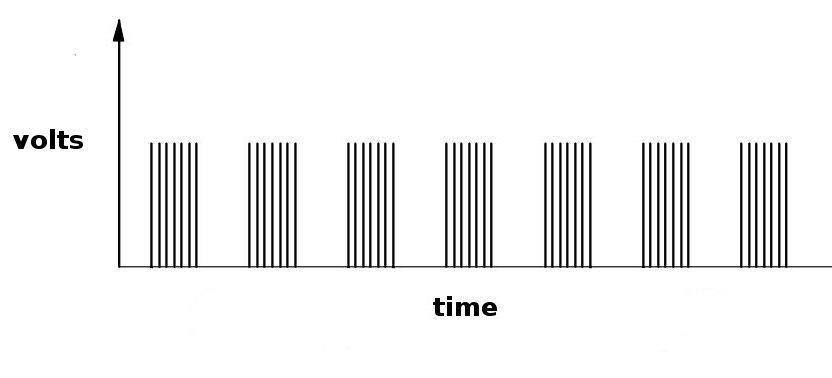
\includegraphics[width=\linewidth]{pic.jpeg}
            \caption{\label{fig:boat}The IR signal}
        \end{figure}
    \subsection{Principles of signal transmission}
        \begin{figure}[ht]
            \centering
            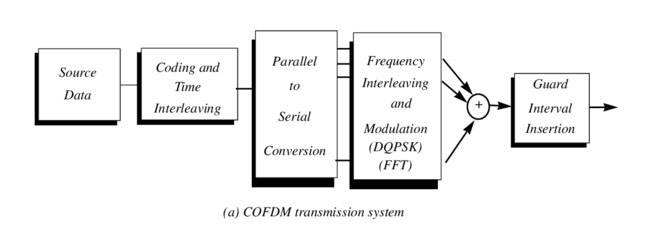
\includegraphics[width=\linewidth]{transmitter.jpg}
            \caption{\label{fig:boat}Principle of transmission}
        \end{figure}
        \newpage
        Explain the diagram: 
        \linebreak
        \par At the transmitter, the message is encoded bit by bit. After the last bit of the message passes, 
        two flushing bits 0 are interested to make sure the last transittion state is 00. Its aim is 
        to facilitate the decoding process of receiver. 
        \linebreak
        \begin{itemize}
            \item Function selection and coding block: when the user presses the function keys to 
            issue the request according to his request, each function key corresponds to the decimal 
            number. The coding circuit will convert into corresponding binary code in the form of a 
            digital signal code consisting of 0 and 1. The number of bits in a binary instruction code 
            maybe 4 or 8 bits depending on the number of function keys more or less.
            \item Conditional oscillator block: when we press a function key, we simultaneously start the 
            oscillator circuit to generate clock pulse, the clock frequency determines the standard time of each bit.
            \item Data latch block and parallel conversion unit to serial: the binary code at the coding circuit 
            will be latched into the parallel data conversion circuit to serial. Serial to parallel data conversion 
            circuits are controlled by clock pulses and timing circuits to ensure a timely completion of the conversion 
            of a sufficient number of bits of code.
            \item Modulation and FM transmitter block: The code in the form of serial will be sent through 
            the modulation circuit and FM transmitter to pair the code into the carrier with the frequency 
            of about 38kHz to 100kHz, thanks to the higher frequency signal carrier, the longer the signal 
            is transmitted, which means increasing its transmitting distance.
            \item Transmitter device block: it is simply an infarred LED. When the instruction code has a bit 
            value of 1, LED imits infarred in the T interval of that bit. When the instruction code has a 
            bit value of 0, LED will not light. Therefore, if the receiver does not receive the signal, it will 
            be considered as having a bit value of 0.
        \end{itemize}
    \newpage
    \subsection{Principles of signal reception}
        \begin{figure}[ht]
            \centering
            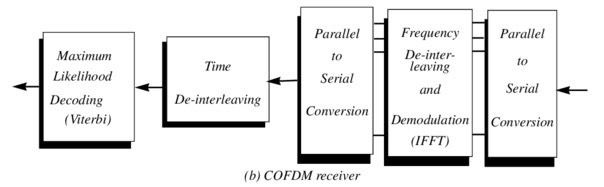
\includegraphics[width=\linewidth]{receiver.jpg}
            \caption{\label{fig:boat}Principle of reception}
        \end{figure}
        \par Explain the diagram:
        \begin{itemize}
            \item Receive unit: infarred from the transmitter is directly received by the infarred 
            receiver or other optical components.
            \item Application and decoupling unit: the signal amplification component will receive 
            first and then pass through the detector circuit to eliminate the carrier and decouple 
            the necessary data, which is the code.
            \item The carrier frequency is also used to compare the phase with the oscillation frequency 
            on the receiver side to help the transceiver circuit be synchronized, ensuring the detector 
            and serial to parallel circuits work correctly.
        \end{itemize}
    \section{Learn about infrared transmitter circuit}
    \begin{figure}[ht]
        \centering
        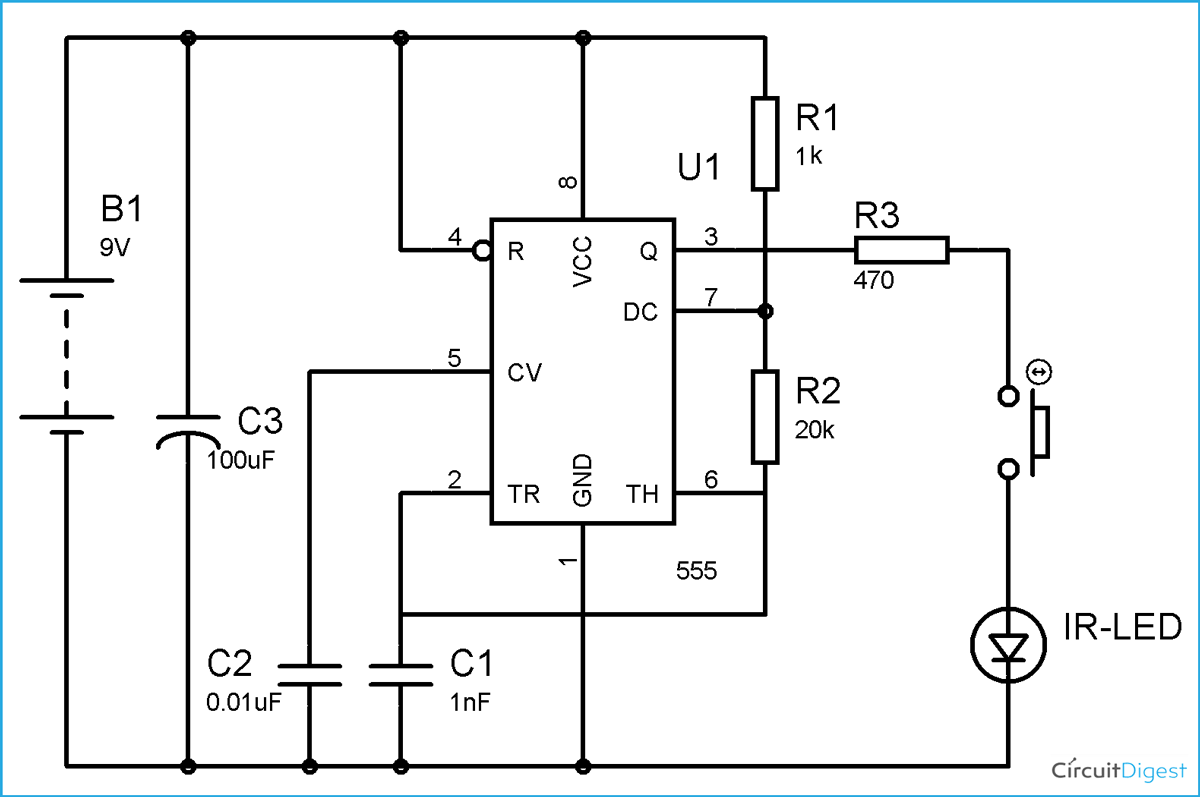
\includegraphics[width=\linewidth]{transmitter.png}
        \caption{\label{fig:boat}Transmitter Circuit Diagram}
    \end{figure}
        \newpage
        Here we use the infrared receiver (TSOP) for the receiver, so we need to create an IR (Infrared Ray) 
        modulated at 38kHz. We can use any receiver, but we need to create IR with the frequency corresponding 
        to the infrared receiver. Therefore, we should use the 555 timer in Astable mode (as above on the section on IC 555 mentioned) 
        to oscillate at 38kHz frequency.
        \linebreak
        \par In this circuit, the oscillator frequency of 555 timer is decided by resistor R1,R2 and capacitor C1. 
        We use 2 resistor R1,R2 and capacitor C1 to create frequency of approximately 38kHz. It is calculated 
        by the following formula: 
        \begin{equation*}
            F = \frac{1.44}{((R1+2*R2)*C1)}
        \end{equation*}
        \linebreak
        \par PIN 3 of IC 555 (timer) is connedted to IR LED by R3 resistor and push button switch. 
        Whenever we press the button, the circuit will emit an infrared signal modulated at 38kHz. 
        Capacitor C1 is responsible for filtering noise for the circuit.
        \newpage
    \section{Learn about infrared receiver circuit}
        \begin{figure}[h]
            \centering
            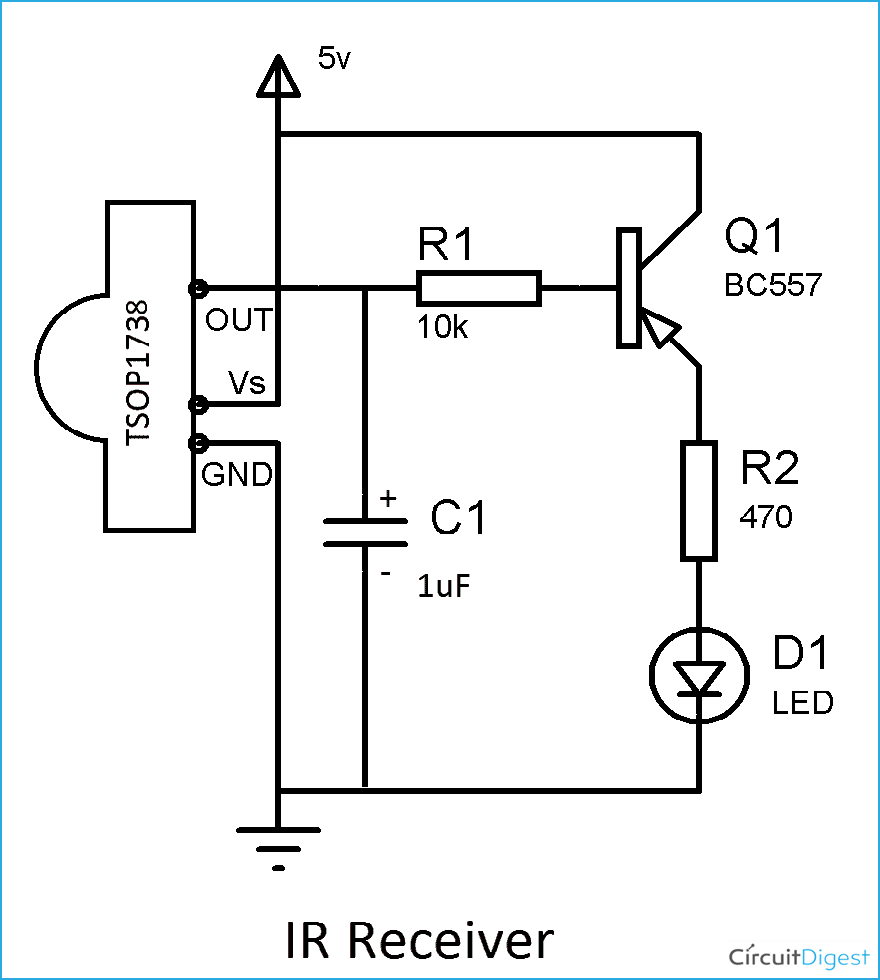
\includegraphics[width=\linewidth]{receiver.png}
            \caption{\label{fig:boat}Receiver Circuit Diagram}
        \end{figure}
        About the receiver circuit is very simple, what all we do is connect a LED to the output of 
        infrared receiver eye 1738 with purpose to check the receiver. Here we use semiconductor light bulb 
        BC557 PNP, the purpose is to reverse the effect of the infrared receiver eye, that mean whenever 
        the output is high, the LED will turn off and vice versa if whenever low, the LED will turn off. 
        PNP transistor work in stark contrast to NPN semiconductor light bulb, it works like a open switch when 
        a voltage is applied to its base and works as a closed switch when there is no voltage as it base. So, 
        usually the output of TSOP still high and transistor works like an open switch and LED will turn off. 
        When the TSOP discovered the infrared, the output will get low and semiconductor light bulb will work 
        like a close switch and LED will turn on. A resistor 10k$\Omega$ usually use to provide appropriate 
        deviation for semiconductor light bulb and resistor 470$\Omega$ use at LED to limit the current.
    \section{Quickview about relay}
        \subsection{Introduction}
            Relay is a passive electronic components usually use in practical application. When we 
            have problem about wattage and we need high stability, besides can be easily to maintenance.
            \linebreak
            \par Relay actually is a switch (also known as K key). But relay different from conventional electrical 
            switch is relay is activate by electric instead of we use the manually is flipped the switch. 
            So, relays are often used as electronic switches. Relay is a switch, so it has 2 status: open and close.
    \subsection{Structure of relay}
        \begin{figure}[ht]
            \centering
            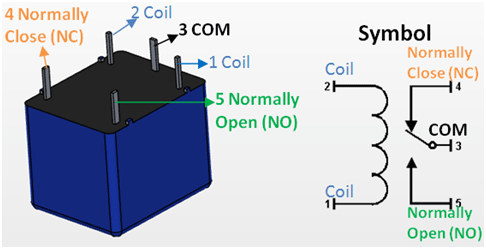
\includegraphics[width=\linewidth]{relay.png}
            \caption{\label{fig:boat}Relay's structure}
        \end{figure}
        \begin{table}[ht]
            \centering
            \begin{tabular}{ | p{2cm} | l | p{5cm} | }
                \hline
                Pin number & Pin name & Description \\ \hline
                1 & Coli end 1 & Used to trigger (on/off) the relay, normally one end is connected to 5V and the other end to ground \\ \hline
                2 & Coli end 2 & Used to trigger (on/off) the relay, normally one end is connected to 5V and the other end to ground \\ \hline
                3 & Common (COM) & Common is connected to one End of the load that is to be controlled \\ \hline
                4 & Normaly Close (NC) & The other end of load is connected to NO or NC. If connected to NC, load still connect before activate \\ \hline
                5 & Normaly Open (NO) & The other end of load is connected to NO or NC. If connected to NC, load still disconnect before activate \\
                \hline
            \end{tabular}
            \caption{\label{tab:sixth}Describe the function of each relay PIN}
        \end{table}
        \vspace{5mm}
    \subsection{Schematic diagram of relay and how it works}
        Relays are most commonly used switching device in electronics. 
        \linebreak
        \par Before we processed with the circuit to drive the relay we have to consider two important parameter of relay. 
        Once is \textbf{Trigger Voltage}, this is the voltage required to turn on the relay that is to change 
        the contact from Common -> NC to Common -> NO. Our relay here have 5V trigger voltage, but you can 
        also find relays of value 3V, 6V even 12V. So select one based on the available voltage in your project. 
        The other parameter is your \textbf{Load Voltage and Current}, this is the amount of voltage or current 
        that the NC,NO or Common terminal of the relay could withstand, in your case for DC it is maximum 
        of 30V and 10A. Make sure the load you are using falls into this range.
        \linebreak
        \begin{figure}[ht]
            \centering
            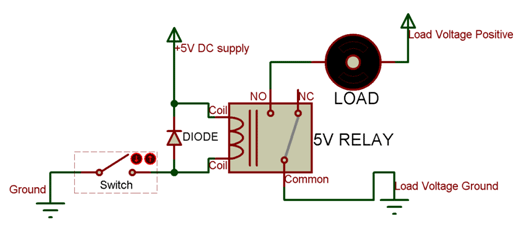
\includegraphics[width=\linewidth]{relay-working.png}
            \caption{\label{fig:boat}Schematic diagram of relay}
        \end{figure}
        \linebreak
        \par The above circuit shows a bare-minimum concept for a relay to operate. Since the relay 
        has 5V trigger voltage we have used a 5V DC supply to the end of coli and other end to ground 
        through a switch. This \textbf{switch} can be anything from a small transistor to a microcontroller 
        or a microprocessor which can perform switching operating. You can also notice a diode connected 
        across the coli of the relay, this diode is called the \textbf{Fly back Diode}. The purpose 
        of the diode is to protect the switch from high voltage spike that can produced by the relay coli. 
        As shown one end of the load can be connected to the Common PIN and the other end is either connected 
        to NO or NC. If connected to NO the load remains disconnected before trigger and if connected 
        to NC the load remains connected before trigger.
    \subsection{Featured of 5-PIN 5V Relay}
        \begin{itemize}
            \item Trigger Voltage (Voltage across coli): 5V DC
            \item Trigger Current (Nominal Current): 70mA
            \item Maximum AC load current: 10A @ 250/125V AC
            \item Maximum DC load current: 10A @ 30/28V DC
            \item Compact 5-PIN configuration with plastic moduling
            \item Operating time: 10msec release time: 5msec
            \item Maximum switching: 300 operating/minute (mechanically)
        \end{itemize}
    \subsection{Types of relays and how to determine their status}
        Currently on the market we have 2 main models: the relay closes at a low level (connect negative pole -> relay close), 
        the relay closes at a high level (connect positive pole -> relay close). If the comparision between 
        2 modules has the same specifications, almost all of its components are the same, except that 
        the transistor of each module. Becasue of this transistor, there are 2 types of relay modules.
        \begin{figure}
            \centering
            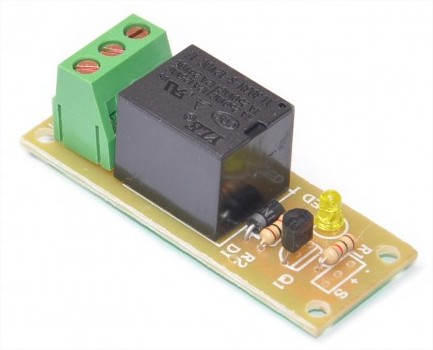
\includegraphics[width=\linewidth]{relay1.jpg}
            \caption{\label{fig:boat}High Quality Relay Model}
            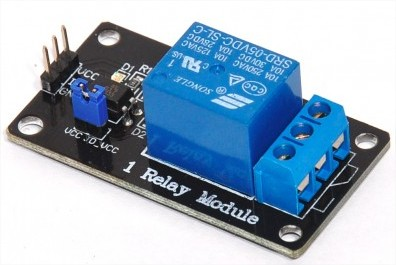
\includegraphics[width=\linewidth]{relay2.jpg}
            \caption{\label{fig:boat}Low Quality Relay Model}
        \end{figure}
        \newpage
    \subsection{Application of relay}
        Relays are widely used and used for a variety of purpose. In which, relays are often used 
        with some basic functions as follow:
        \begin{itemize}
            \item Switching multiple currents or voltage to different loads using a control signal.
            \item Monitor industrial safety systems and disconnect machinery if safety is ensured.
            \item And the more practical application, when running on the road you need to turn left, 
            now you will need the flashing signal from the turn signal light, even the click-click. What make that sound is relay.
        \end{itemize}
    \section{Quickview about mini pulse source module}
        \begin{figure}[ht]
            \centering 
            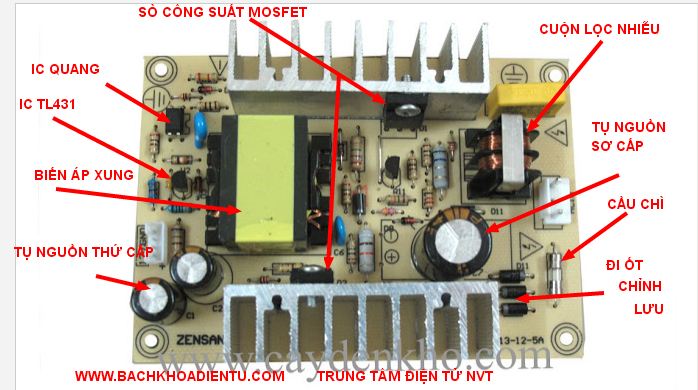
\includegraphics[width=\linewidth]{nguon xung.png}
            \caption{\label{fig:boat}The actual pulse source circuit is often used}
        \end{figure}
        We have often heard the term "pulse source" a lot, but most of us don't know what it is. 
        It includes any component and its superiority in electronic design. The application of pulse 
        sources is usually very wide, it will appear in devices such as: induction hob, microwave oven, 
        electric cooker, amplifier, hood, electric fan... So what is the source of the pulse? This will be 
        basic information about pulse source.
    \subsection{What is pulse source?}
        Impulse source is a power supply unit that converts from an alternating current source to 
        a direct current by means of an oscillating mode created by electronic circuits combined with 
        a pulse transformer, and other basic components.
    \subsection{Structure of the pulse source circuit?}
        Common pulse sources are made up of basic components as follows:
        \begin{itemize}
            \item Pulse transformer: Made from coil wound on a magnetic core similar to the conventional 
            transformer we often use. Pulse transformer usually use ferritic cores and have quite a large 
            capacity, it can work well even in the high frequency range, things that conventional transformer 
            can hardly meet.
            \item Fuse: the effect of a common fuse to protect the power circuit from short circuit.
            \item Anti-jamming coil, primary filter capacitor, rectifier diode: these things are responsible 
            for converting the 220V AC voltage into the DC voltage stored on the primary filter capacitor to 
            power the primary winding of the pulse transformer machine.
            \item Power shell: this is a semiconductor component used as a switch, which can be a transistor, 
            mosfet, integrated IC, IGBT (Transistor with isolation control pole) is responsible for cutting 
            power from positive pins of the primary filter capacitor on the primary winding of the pulse transformer 
            and then dropped to mass.
            \item Secondary power filter capacitor: it is used to store electrical energy from the secondary 
            winding of the pulse transformer to supply comsumption. We know that when the primary winding of 
            the transformer is continuously switched on by the power cockle, the reciprocal magnetic field appears, 
            which leads to the secondary winding of the transformer. This voltage is rectified through several diodes 
            and then out put secondary filter capacitor to flatten the voltage.
            \item Optical IC and TL431 ICs: these 2 ICs are responsible for creating a fixed voltage to control 
            the voltage on the secondary side stable as we wish. They will control the switching on the primary 
            winding of the transformer so that the secondary output is satisfactory. 
        \end{itemize}
    \subsection{Block diagram and principle of operation of the pulse source}
        \begin{figure}[ht]
            \centering
            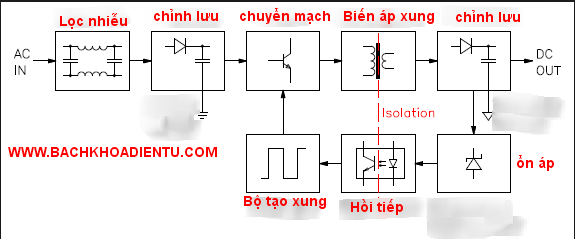
\includegraphics[width=\linewidth]{diagram.png}
            \caption{\label{fig:boat}Block diagram of pulse source}
        \end{figure}
        First the input voltage is from 80V to 220V AC through the noise filter coil and then into the rectifier 
        diode into DC about 130-300V (depending on AV voltage at the input) on the primary filter capacitor. 
        The primary filter capacitor. The primary filter capacitor is responsible for the storage of DC power 
        for the transformer primary pulse operating coil. The common primary filter capacitors will have 
        value such as: 4.7$\mu$F-400V, 10$\mu$F-400V, 220$\mu$F-400V, 10$\mu$F-200V.
        \linebreak
        \par The primary winding of the pulse transformer is energized according to the high frequency pulse 
        through the semiconductor switching block, which is components such as transistor, mosfet or IGBT 
        (Transistor with isolated control pole). These electrical impulses are generated by a pulse generator 
        or electronic oscillating circuits.
        \linebreak
        \par In the secondary winding: the secondary winding of the pulse transformer will have rectifier 
        circuits that give a direct current to power to load. This secondary voltage will be maintained at 
        a certain voltage such as 3.3V, 5V, 9V, 12V, 15V, 18V or 24V thanks to the voltage stabilizer circuit. 
        At the same time, the feedback circuit will take out the voltage signal to put into the oscillator 
        to control so that the oscillation frequency is stable with the ouput voltage as we want. The voltage 
        regulator IC is often used as: 7805, 7809, 7812, 7818. The PIN IC inserted into the feedback circuit 
        is IC431, while the main feedback IC is the Opto couple PC817.
    \subsection{Some basic types of pulse sources}
        \begin{itemize}
            \item Buck type: transform the source for a smaller output voltage than the input voltage is Vinout.
            \item Boot type: for ouput voltage greater than input voltage Vin < Vout.
            \item Flyback type: indirect power transmission via transformer. Output voltage is greater or smaller 
            than input voltage. And especially from an input, it can produce a lot of output voltage. 
            \item Push-Pull type: also known as push pull. This type of impulse source is transmitted indirectly 
            through a transformer, giving an output voltage smaller or larger than the input voltage. And just like 
            with Flyback type, from one type of input voltage can produce many output voltages.
        \end{itemize}
        In this content, we will use a mini pulse source that converts from AC 220V AC to 5V DC and the 
        maximum power is 3W, the design of this circuit uses AC/DC isolation pulse transformer and Anti-interference 
        and feedback machanisms for maximum safety and stability. 
        \begin{figure}[ht]
            \centering
            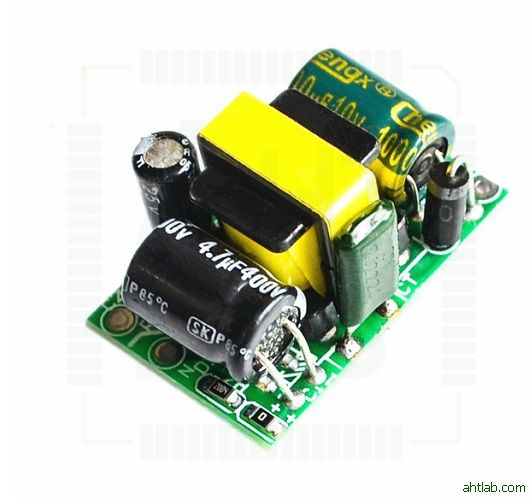
\includegraphics[width=0.5\linewidth]{pic1.jpg}
            \caption{\label{fig:boat}5V-3W pulse power model}
        \end{figure}
        The specifications of this module are as follows: 
        \begin{itemize}
            \item Input voltage: 85-256V AC
            \item Input current: 0.0273A (110V AC) / 0.014A (220V AC)
            \item Output voltage: 5V DC (error 1\%)
            \item Average output current: 600mA
            \item Wattage: 3W
            \item Size: 20 x 30mm
        \end{itemize}
    \section{Remote Controlled circuit}
        \subsection{Circuit principle}
            \begin{figure}[ht]
                \centering
                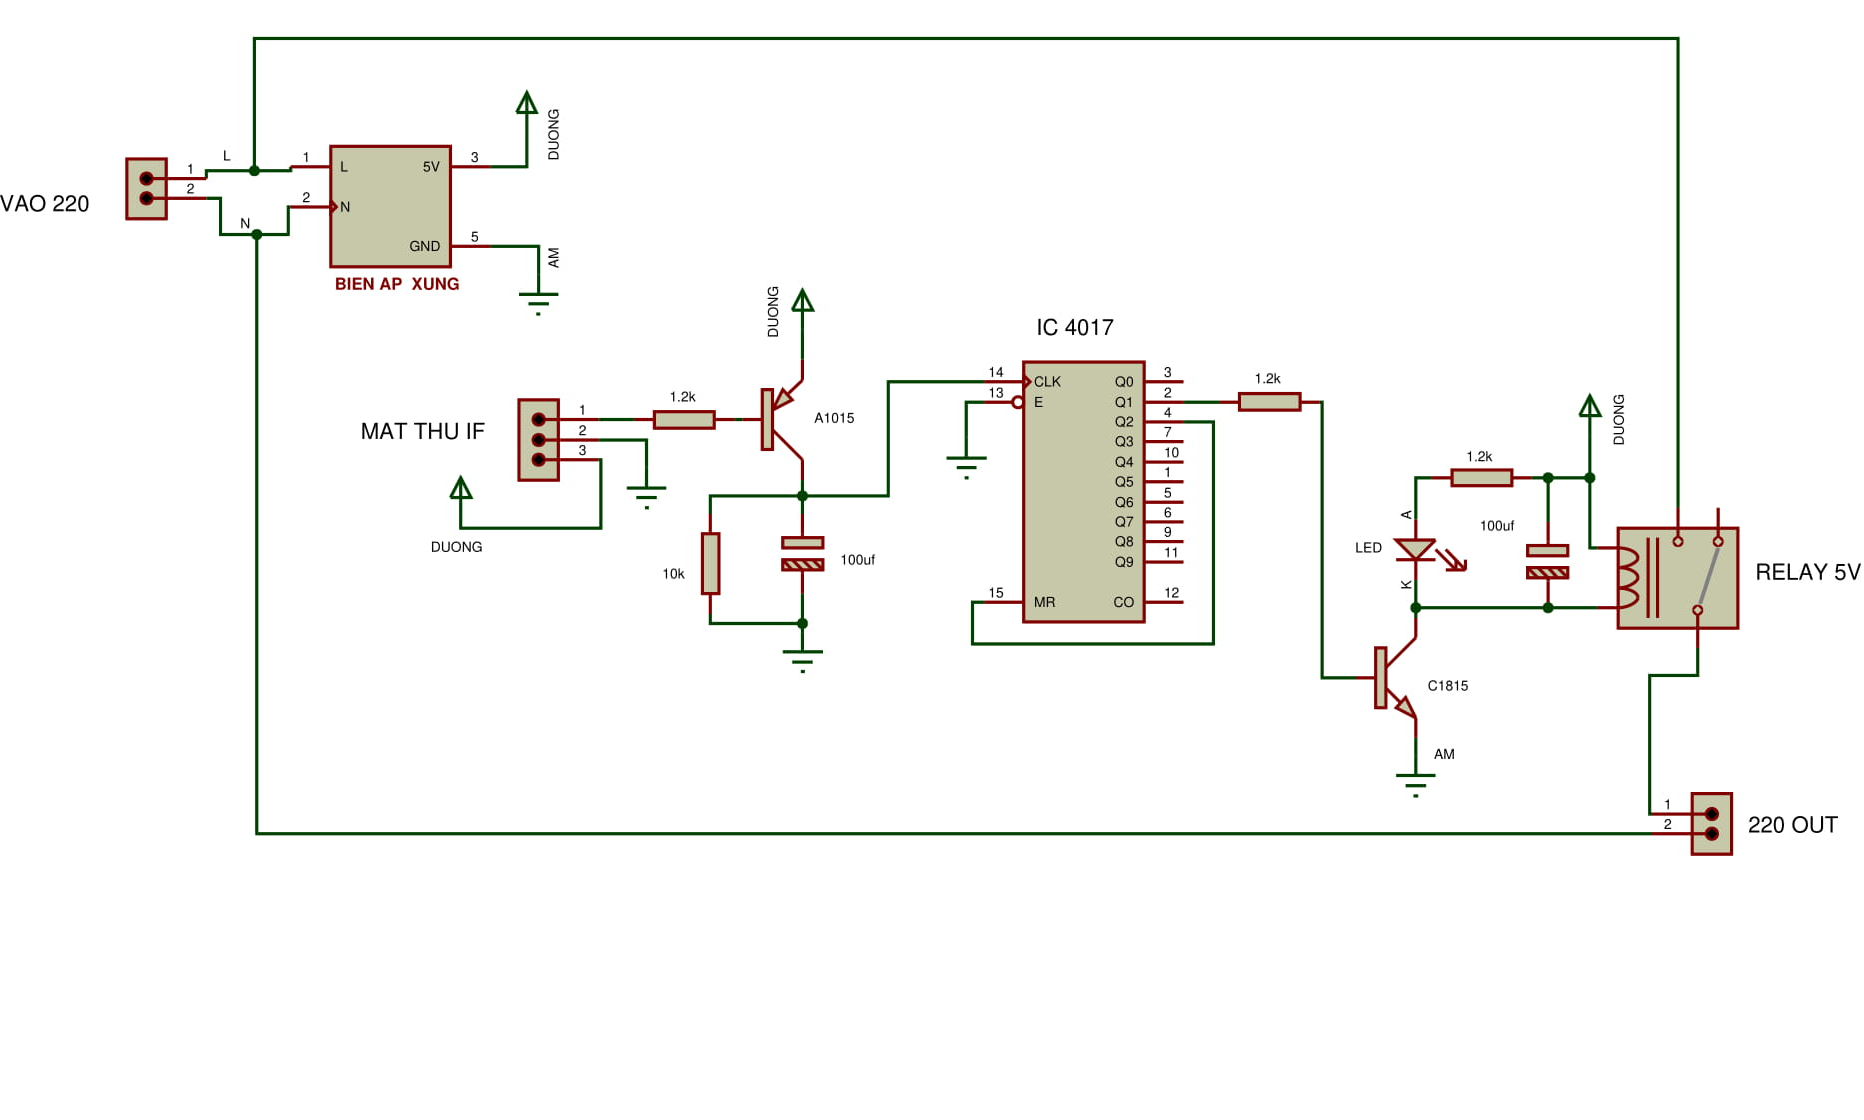
\includegraphics[width=\linewidth]{pic1.png}
                \caption{\label{fig:boat}Principle remote control circuit}
            \end{figure}
        \subsection{Explain the principle of circuit}
            The mini pulse transformer converts from 220V AC to 5V DC, the positive and negative positions in 
            the circuit are connected together. When transmitting the signal to the infrared receiver (TSOp) 
            from which TSOP will generate a signal at the signal pin of the infrared receiver, then A1015 transistor 
            leads and fills capacitor C5 according to the principle of the capacitor, the capacitor will discharging 
            through resistor R7 will produce a shock at pin 14 of IC 4017. Therefore, the signal generated from pin 
            number 3 transmits to pin number 2 to a high level. The C1815 resistor is activated to make the relay 
            work in principle. So the load will work with AC voltage of 220V.
            \linebreak
            \par Similarly, once we trigger the signal in the infrared receiver again, it is similar to the first 
            time it generates a pulse at pin number 14 of IC 4017, and it will restart the output signal at pin number 2 
            to low level, C1815 transistor will not lead to a failure of the relay. So the load will not work.
    \chapter{Construction circuit and results}
    \thispagestyle{fancy}
    \fancyhf{}
    \fancyhead[L]{CaptainJAV}
    \fancyhead[R]{Remote Controlled Using Infarred}
    \rfoot{Page \thepage}

    \chapter{Conclude}
    \thispagestyle{fancy}
    \fancyhf{}
    \fancyhead[L]{CaptainJAV}
    \fancyhead[R]{Remote Controlled Using Infarred}
    \rfoot{Page \thepage}
    \begin{itemize}
        \item The circuit works exactly as the target set.
        \item Advantages: The circuit is quite simple and easy to do, the principle as well as finding data are quite simple.
        \item Disadvantages: Using a lot of components, wires (if do it on Vero board), cost is quite a lot, must test on the test board many time to get the desired results.
    \end{itemize}

    \newpage
    \thispagestyle{plain}
    \centerline{\textbf{\huge{REFERENCES}}}
    \vspace{10mm}
    \begin{enumerate}
        \item Jayant (Oct 20, 2015), IR Transmitter and Receiver
        \item Jayant (Oct 18, 2015), Remote Controlled Light Switch
        \item Mai Thanh An, Remote Controlled using Infrared 
        \item Anusha (Apr 22, 2017), Remote Controlled Light Switch
        \item Dr.Ho Ngoc Ba (2013), Electronic Circuit curriculum similar
    \end{enumerate}
\end{document}